% ------------------------------------------------------------------------------
% Metodologia
% ------------------------------------------------------------------------------

\chapter{Metodologia}\label{chap:metodologia}

Como fundamento do desenvolvimento desse trabalho, está a utilização das técnicas de ES para tornar o dia-a-dia de trabalho e gestão de atividades mais claros e concisos. Além disso, busca-se a especificação das deficiências no processo ou ciclo de vida que, apesar de já serem percebidas, não estão bem colocadas ou esclarecidas.

A primeira etapa de trabalho consiste na definição do ciclo de vida como é hoje. Através do estudo do fluxo atual, são definidas as associações das etapas elencadas com as fases de cada estágio do ciclo de vida da ES, bem como seus entregáveis e os pontos de decisão entre elas. Recapitulando, o serviço prestado é basicamente o desenvolvimento de diferentes sistemas para atender requisitos específicos das áreas de negócios trazidos ao time.

Para complementar esse ciclo de vida, é desenvolvida a arquitetura dos elementos do sistema e estabelecida a relação entre eles e com as funcionalidades. Assim, são definidas todas as opções de possíveis sistemas do serviço prestado, através das combinações de elementos do sistema e das funcionalidades.

Após essa primeira parte do trabalho, com os artefatos e documentações já produzidas, é feita a análise e listagem dos problemas e deficiências encontradas no ciclo de vida. Tendo em mãos os problemas identificados, são feitas propostas para saná-los ou amenizá-los, sendo detalhado como e o que deve ser feito, quais materiais ou instrumentos são utilizados, e o que se espera com a proposta sugerida.

Por fim, propõe-se uma coleta de resultados para a análise e avaliação do trabalho realizado.

	\section{Ciclo de Vida}

	Inicialmente definiu-se em formato de fluxograma o processo do serviço prestado, para dessa forma ser 
	mais fácil o entendimento da ordem das etapas. Depois traremos essa representação para o formato esperado
	na ES. A Figura \ref{fig:metodologia:processFlow} mostra esse fluxograma.
	
	\begin{figure}[!tb]
		\centering
		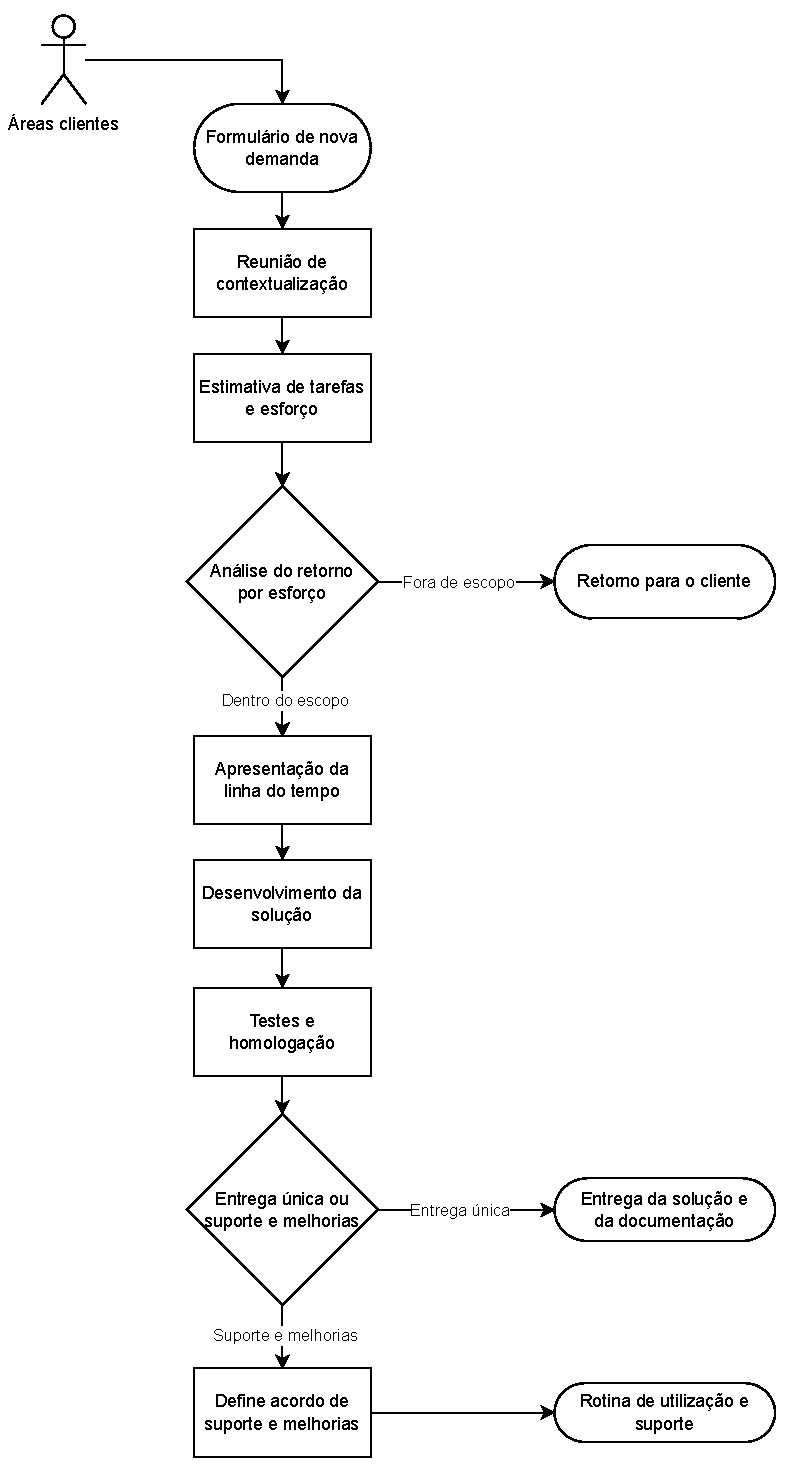
\includegraphics[width=0.6\textwidth]{./figuras/processFlow.pdf}
		\caption{Fluxograma do processo que descreve o serviço prestado.}
		\label{fig:metodologia:processFlow}
	\end{figure}
	
	Cada um dos blocos do fluxograma representa uma etapa do processo, e cada etapa é descrita abaixo:
	\begin{itemize}
		\item \textbf{Formulário de novo desenvolvimento}
		\begin{itemize}
			\item Descrição: Esse formulário é o ponto de entrada de uma nova demanda para o time. Quando uma área
			cliente manifesta a necessidade e procura o auxílio do time, ela é direcionada a responder esse formulário
			online com uma série de perguntas. E há ainda, casos em que auditorias internas encontram irregularidades em processos existentes,
			e os encaminham para entrar em contato com o time para possíveis soluções de remediação, novamente eles são direcionados para responder o formulário.
			\item Objetivos: Obter informações de contato e departamento do requisitante bem como o centro de custo em caso de
			possíveis cobranças no futuro. Levantar informações iniciais sobre a solução desejada como classificação dos dados envolvidos, 
			interdependência com outras áreas e quais dores seriam sanadas com o desenvolvimento.
			Coletar dados e percepções que ajudem a mensurar o valor para a área e para a empresa como um todo, ao ser desenvolvida uma
			solução para essa demanda. Solicitar documentação disponível do processo atual caso exista.
			\item Saídas: Registro das respostas ao formulário, anexos e documentações enviadas.
		\end{itemize}
		\item \textbf{Reunião de contextualização}
		\begin{itemize}
			\item Descrição: Após recebida e revisada a resposta do formulário, o gerente de projetos organiza essa reunião com os desenvolvedores
			envolvidos e o requisitante, orientando-o a convidar todas as outras partes interessadas. Nessa reunião, o requisitante faz uma nova explicação dos problemas e possíveis
			de soluções, e também são sanadas possíveis dúvidas sobre as respostas do fomulário e sobre a documentação enviadas anteriormente.
			\item Objetivos: Entender o papel de todas as partes interessadas na operação. Ver o processo atual existente sendo executado integralmente
			pelos responsáveis. Obter exemplos de artefatos do processo como emails enviados, arquivos gerados ou compartilhados,
			indicadores calculados e outros artefatos que sejam importantes, caso existam. Discutir casos de uso e cenários que não existem atualmente
			mas são desejáveis na solução. Discutir políticas de retenção de dados.
			\item Saídas: Gravação da reunião e operação atual. Arquivos com os exemplos de artefatos do processo atual.
		\end{itemize}
		\item \textbf{Estimativa de tarefas e esforço}
		\begin{itemize}
			\item Descrição: Nessa etapa os desenvolvedores de maior senioridade realizam uma sintetização das necessidades e requisitos para propor
			um ou mais cenários de solução. Assim, em um curto espaço de tempo, são definas histórias de usuário em um alto nível, sem muito detalhamento,
			para que seja estimado o esforço e tempo total necessário para o desenvolvimento dos cenários de solução. 
			\item Objetivos: Definir cenários de solução para o caso trazido pelo cliente. Estimar o esforço e tempo necessário para executar as tarefas definidas para cenário.
			\item Saídas: Documento com cenários propostos, tempo e esforço necessários para cada um. 
		\end{itemize}
		\item \textbf{Análise do retorno por esforço}
		\begin{itemize}
			\item Descrição: Ao receber o documento da etapa anterior o gerente de projetos de reúne com o gerente e o diretor da área,
			onde realizam uma análise de enquadramento de escopo de todas as submissões que estão aguardando o início do desenvolvimento, e 
			depois uma priorização das que serão iniciadas. Essa etapa é realizada em uma menor frenquência,
			geralmente bimestralmente, salvo exceções em que envolvem uma falha em auditoria e que precisam de mais celeridade.
			\item Objetivos: Definir se a demanda solicitada está no escopo do time (dentro das capacidades técnicas do time, dentro do tempo máximo de desenvolvimento por projeto, não conter
			dados estritamente confidenciais, gerar um valor que valha o investimento). Priorizar a ordem de execução das tarefas.
			\item Saídas: Lista com os projetos selecionados e priorizados para execução.
		\end{itemize}
		\item \textbf{Retorno para o cliente}
		\begin{itemize}
			\item Descrição: Quando um projeto é definido como fora de escopo, é marcada uma reunião com o requisitante e apresentado 
			os motivos da decisão. A depender do motivos são passadas orientações para a área cliente, como procurar outro time de desenvolvimento interno na empresa,
			utilizar uma ferramenta existente no mercado, contratar time externo para executar o projeto, ou mesmo redefinir os requisitos e necessidades e submeter novamente para análise.
			Essa etapa é um dos possíveis fins do fluxo de serviço.
			\item Objetivos: Apresentar uma devolutiva ao requisitante da demanda. Orientar sobre possíveis alternativas.
			\item Saídas: Ata da reunião com principais tópicos, decisões, e participantes.
		\end{itemize}
		\item \textbf{Apresentação da linha do tempo do projeto para o cliente}
		\begin{itemize}
			\item Descrição: Quando um projeto é definido como dentro do escopo e priorizado, é marcada uma reunião com o requisitante
			para dar um retorno sobre essa priorização. O gerente de projetos apresenta como ficou a linha do tempo estimada para os diferentes cenários e quando será
			iniciado o desenvolvimento.
			\item Objetivos: Apresentar o cronograma e início do desenvolvimento. Definição de qual cenário será desenvolvido. Coletar possíveis ressalvas quanto aos prazos informados.
			Definir agendas para acompanhamento do progresso do desenvolvimento.
			\item Saídas: Ata da reunião com principais tópicos, decisões, e participantes. Agenda com as reuniões de acompanhamento.
		\end{itemize}
		\item \textbf{Desenvolvimento da solução}
		\begin{itemize}
			\item Descrição: Esta é a etapa dedicada ao trabalho de desenvolvimento de programação da solução proposta e escolhida. A partir das histórias de usuário
			criadas anteriormente, semanalmente são criadas taferas detalhando as atividades a serem realizadas na próxima semana para cada história de usuário.
			\item Objetivos: Detalhar as histórias de usuário em tarefas. Executar as tarefas de cada história de usuário.
			\item Saídas: Solução desenvolvida com todas as suas fucionalidades.
		\end{itemize}
		\item \textbf{Teste e homologação}
		\begin{itemize}
			\item Descrição: Ao ser finalizado o desenvolvimento da solução é realizada um demonstração ao requisitante e às partes interessadas.
			A solução é implantada no ambiente de qualidade para que os usuários façam testes e validem se as funcionalidades e requisitos foram cumpridos.
			Em paralelo o time de desenvolvimento trabalha para corrigir problemas encontrados.
			\item Objetivos: Usuários validarem as funcionalidades da solução desenvolvida. Corrigir possíveis problemas encontrados. Definir uma data para fim dos testes em qualidade. 
			\item Saídas: Relatório de problemas encontrados na ferramenta. Relatório com possíveis melhorias futuras. Relatório com as correções realizadas.
		\end{itemize}
		\item \textbf{Entrega única ou suporte e melhorias}
		\begin{itemize}
			\item Descrição: Nessa etapa se inicia o encerramento do projeto. É realizada uma reunião com o requisitante e as partes interessadas, onde discute-se
			sobre como foi o andamento do projeto e são explicadas as opções de continuidade para a área cliente demandante. Onde existem as opções de contratarem 
			um plano de suporte e melhorias com o time de desenvolvimento ou seguirem por conta própria com a solução desenvolvida. 
			\item Objetivos: Formalizar a entrega da solução desenvolvida. Apresentar com mais detalhes as opções de continuidade. Estipular um prazo para retorno sobre qual será a opção escolhida, caso não seja decidido na reunião.
			\item Saídas: E-mail com a formalização da entrega. Prazo para decisão dos próximos passos.
		\end{itemize}
		\item \textbf{Envio do pacote da solução e entrega da documentação}
		\begin{itemize}
			\item Descrição: Caso o requisitante e sua área decidam por não contratar o pacote de suporte e melhorias, são enviadas por e-mail as intruções de como dar continuidade à operação da solução, bem como o pacote contendo a própria solução desenvolvida. Espera-se um atestado de recebimento or parte do requisitante.
			\item Objetivos: Enviar documentação fucional da solução desenvolvida. Enviar pacote com a solução desenvolvida.
			\item Saídas: E-mail com os documentos de entrega do projeto. Atestado de recebimento dos arquivos, que simboliza o encerramento do projeto.
		\end{itemize}
		\item \textbf{Acordo de suporte e melhorias}
		\begin{itemize}
			\item Descrição: Ao optar por seguir com o pacote de suporte e melhorias, são definidas as horas mensais dedicadas e valor a ser pago para esse pacote. Além disso, é demonstrado como são abertas requisições de suporte e melhorias.
			\item Objetivos: Definir horas e custos mensais do pacote se suporte e melhorias. Obter autorização para débito no centro de custo da área cliente.
			\item Saídas: E-mail com acordo de suporte e melhorias.
		\end{itemize}
		\item \textbf{Rotina de manutenção e suporte}
		\begin{itemize}
			\item Descrição: A aplicação é implantada no ambiente produtivo e liberada para operação aos usuários.
			\item Objetivos: Implantar a solução em produção. Encerrar o projeto de desenvolvimento. Iniciar suporte e manutenção da solução.
			\item Saídas: E-mail com intruções de acesso e utilização da ferramenta. E-mail com as instruções para criação de requisições de suporte.
		\end{itemize}
	\end{itemize}

	Para as áreas que não optaram por seguir com um acordo de suporte e melhorias, caso seja necessário uma nova implementação ou modificação relacionada à solução desenvolvida, deverão responder novamente o formulário e passar por todo o processo de análise de retorno por investimento e priorização, como uma nova demanda.
	Já as que tem o acordo de suporte e melhorias, podem utilizar as horas mensais e fazer o balanceamento das mesmas para realizar essas implementações sem passar por todo o processo. Entretanto, mesmo com o acordo, caso seja uma modificação muito grande ou uma nova funcionalidade que demande muito tempo de desenvolvimento, é necessário responder o formulário e iniciar como uma nova demanda ao time, porém ao fim não precisam de um novo acordo de suporte e melhorias, pois já o possuem.

	Trazendo o ciclo de vida em ``V'' mencionado anteriormente, as áreas que possuem o contrato de suporte percorrem todas os estágios, dos dois lados do ``V''. Já as outras áreas,
	param na primeira metade.

	\subsection{Adequação de representação}

	Tendo todas as etapas do processo sido explicadas, são feitas sua relações com os estágios e fases do ciclo de vida proposto na engenharia de sistemas.
	De maneira descritiva, sem ainda avaliar a otimização ou melhoria do ciclo de vida, podemos representar o ciclo de vida com as figuras \ref{fig:metodologia:currentConceptPhases}, \ref{fig:metodologia:currentDevelopmentPhases} e \ref{fig:metodologia:currentPostDevelopmentPhases}.
	
	\begin{figure}[h]
		\centering
		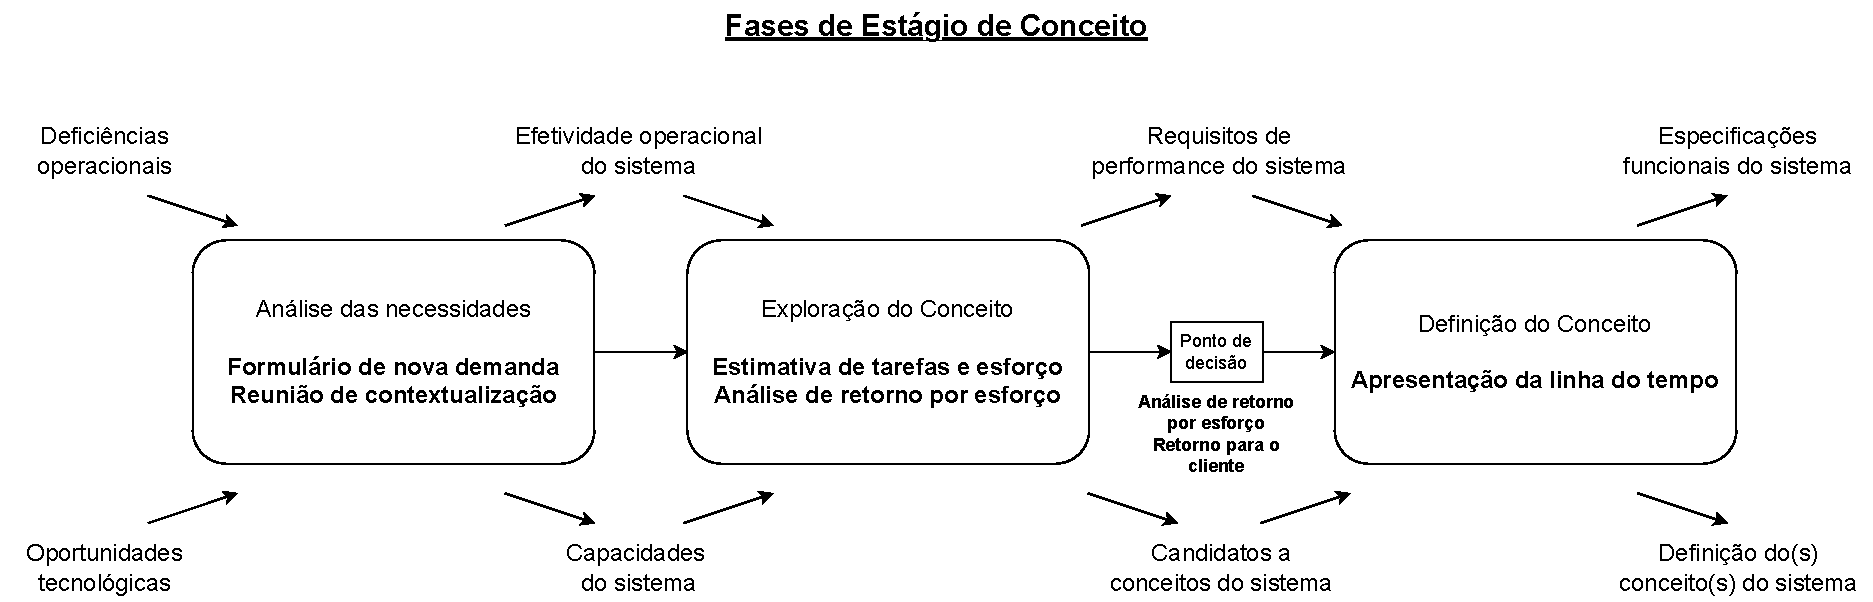
\includegraphics[width=\textwidth]{./figuras/currentConceptPhases.pdf}
		\caption{Relação com as fases do estágio de Conceito}
		\label{fig:metodologia:currentConceptPhases}
	\end{figure}

	Olhando para o estágio de Conceito na figura \ref{fig:metodologia:currentConceptPhases}, na fase de \textbf{Análise das necessidades} temos as etapas
	de \textbf{Fomulário de nova demanda} e \textbf{Reunião de contextualização}. De fato, nessas etapas é realizado o primeiro contato com as áreas 
	clientes e visto a operação que se deseja digitalizar ou otimizar. De forma macro já é entendida as principais capacidades do sistema bem como uma pré-análise de quais tecnologias utilizar.

	Agora na fase de \textbf{Exploração do Conceito} foram alocadas as etapas de \textbf{Estimativa de tarefas e esforço} e \textbf{Análise de retorno por esforço}. A etapa de
	\textbf{Estimativa de tarefas e esforço} já começa a documentar alguns requisitos e separar subsistemas para mensuração de esforço de desenvolvimento, nela são propostas mais de uma abordagem
	de solução quando aplicável e também é analisada a viabilidade técnica. A etapa de \textbf{Análise de retorno por esforço} também
	foi posicionada nessa fase pois nela ocorre a análise de viabilidade estratégica de desenvolvimento do sistema.

	Foi destacado ainda o ponto de decisão entre a fase de \textbf{Exploração do Conceito} e de \textbf{Definição do Conceito}, que é justamente após a análise de viabilidade
	estratégica. Nesse ponto, é decidido se será empenhado mais esforço a fim de continuar o trabalho para o desenvolvimento da solução ou o cancelamento da iniciativa, interrompendo o ciclo
	de vida de avançar, acontece nesse caso a etapa de \textbf{Retorno ao Cliente}.

	Na fase de \textbf{Definição do Conceito} temos a etapa de \textbf{Apresentação da linha do tempo}, pois nessas apresentação são sugeridas as alternativas de desenvolvimento que satisfaçam
	os requisitos estabelecidos, de maneira integral ou não, e suas justificativas para serem utilizadas.
	
	\begin{figure}[h]
		\centering
		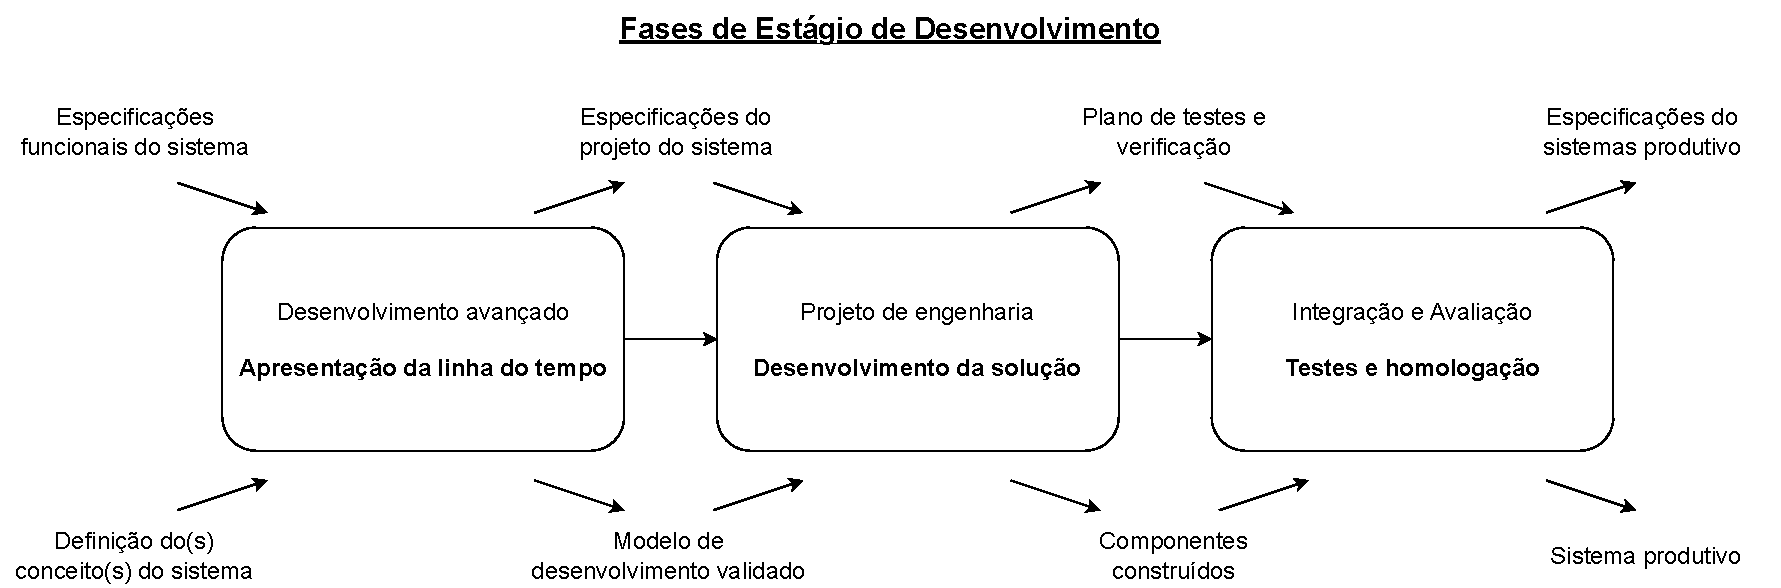
\includegraphics[width=\textwidth]{./figuras/currentDevelopmentPhases.pdf}
		\caption{Relação com as fases do estágio de Desenvolvimento}
		\label{fig:metodologia:currentDevelopmentPhases}
	\end{figure}

	Voltando a atenção para o estágio de Desenvolvimento, na primeira fase de \textbf{Desenvolvimento Avançado} temos novamente a etapa de \textbf{Apresentação da linha do tempo}, pois é realizada
	a apresentação das histórias de usuário, buscando a validação das partes interessadas. São apresentadas as principais funcionalidades junto com a programação de desenvolvimento e também discutido
	o cronograma, captando os riscos do mesmo, no ponto de vista dos outros interessados.

	Na fase de \textbf{Projeto de Engenharia} se encontra a etapa de \textbf{Desenvolvimento da solução}, é feita a programação dos componentes do sistema através das histórias de usuário definidas semanalmente.
	Nesse caso os desenvolvedores e engenheiros empenham os esforços nos componentes onde são especialistas, e depois de desenvolvidos os testam individualmente.

	Por fim, na fase de \textbf{Integração e avaliação} está alocada a etapa de \textbf{Testes e Homologação} visto nessa etapa é realizada a integrações entre os componentes e os testes juntamente com a
	área demandante e um grupo pequeno do time operacional para simular o dia a dia de utilização da solução. São avaliadas a qualidade e completude das
	funcionalidades pré-estabelecidas anteriomente, e uma avaliação geral do escopo do sistema.

	\begin{figure}[h]
		\centering
		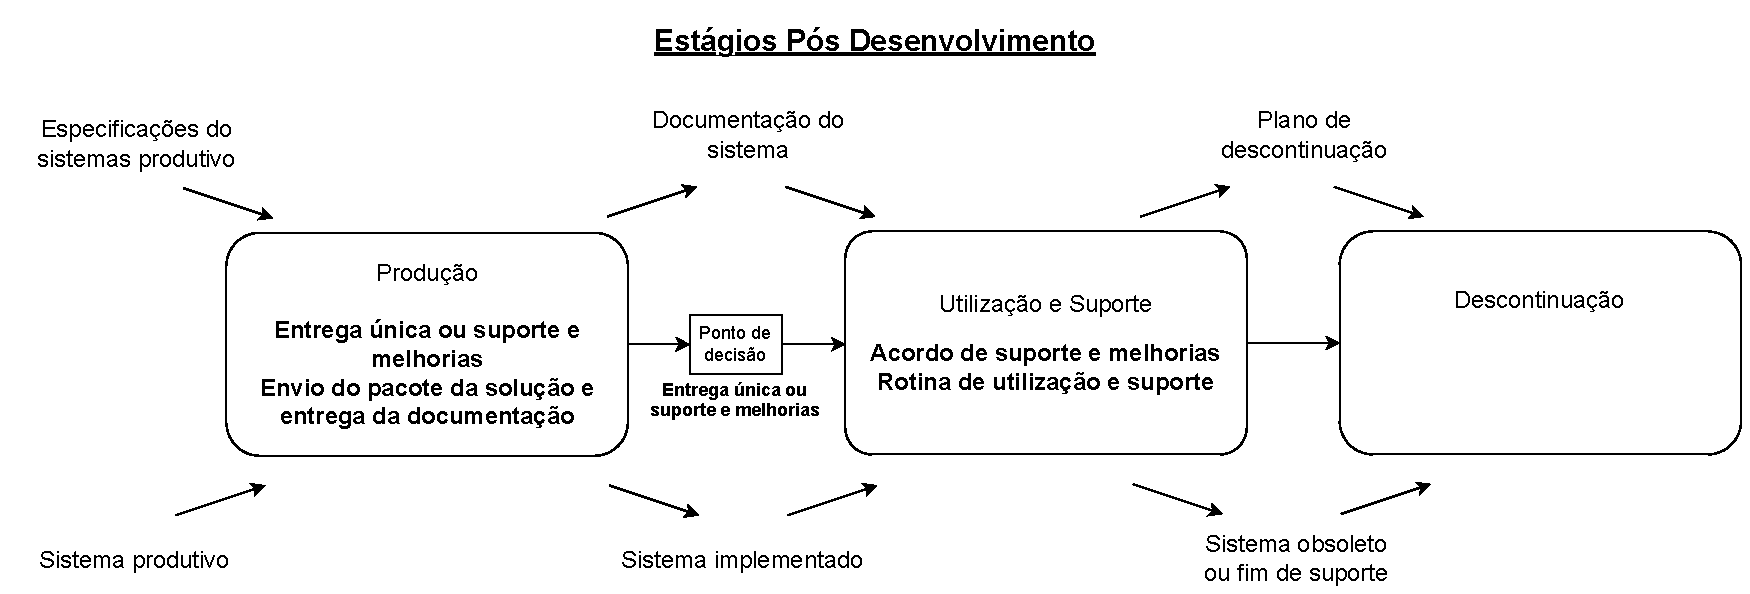
\includegraphics[width=\textwidth]{./figuras/currentPostDevelopment.pdf}
		\caption{Relação com os estágios Pós-Desenvolvimento}
		\label{fig:metodologia:currentPostDevelopmentPhases}
	\end{figure}

	Nos estágios de pós-desenvolvimento, em \textbf{Produção} temos as etapas de \textbf{Entrega única ou suporte e melhorias} e \textbf{Envio do pacote da solução e entrega da documentação},
	na primeira ocorre o aceite da entrega da solução/sistema e após isso é realizado a implantação do sistema em ambiente produtivo.
	Nesse ponto a documentação do sistema também deve estar feita e disponibilizada. Uma nuance do estágio de produção ocorre de acordo com a decisão tomada pela area cliente na etapa \textbf{Entrega única ou suporte e melhorias}, pois caso não optem
	pelo plano de suporte e melhoria, a implantação do sistema ocorre em um ambiente gerenciado por eles, e não pelo time de desenvolvimento, e por isso ocorre a etapa \textbf{Envio do pacote da solução e entrega da documentação}.

	É destacado outro ponto de decisão, entre o estágio de \textbf{Produção} e o de \textbf{Utilização e Suporte}, pois como dito, o ciclo de vida continua apenas se for feito a contração do serviço de suporte.
	Ressaltando que o sistema vai ser utilizado, mas deixa de ser responsabilidade do time de desenvolvimento.

	O estágio de \textbf{Utilização e Suporte} compreende as etapas de \textbf{Acordo de suporte e melhorias} e \textbf{Rotina de utilização e suporte}, onde os usuários, já utilizando o sistema, relatam falhas, problemas e melhorias que são corrigidas
	ou implementadas ainda nesse estágio, ou seja, a segunda metade do ciclo de vida em ``V''.

	Ainda não existe uma etapa criada para \textbf{Descontinuação}, sendo que o time é relativamente novo com cerca de dois anos de criação
	não houve caso de obsolescência mapeado até então.

	\subsection{Avaliação do ciclo de vida}

	Ao longo da repetição desse ciclo de vida para cada solução desenvolvida, já havia sido notado um deficiência
	na parte de definição e validação de conceito. Por vezes, já no fim da fase de \textbf{Projeto de Engenharia} ou durante a fase de \textbf{Integração e avaliação}
	eram identificadas funcionalidades essenciais que não havia sido mapeadas, ou ainda um desenvolvimento que tecnicamente funcionava mas que desempenhava uma 
	funcionalidade desalinhada com a real intenção das partes interessadas.

	Olhando para a representação do ciclo de vida de acordo com as definições da ES, fica mais claro identificar a raiz dessa deficiência bem como o que
	pode ser feito para mudar. A transição entre os estágios de Conceito e Desenvolvimento, marcado pelas fases de Definição de Conceito e Desenvolvimento Avançado, apresenta
	uma falta de artefatos ou documentos que permitiriam essa transição de forma suave mas concisa.

	Um ponto relevante é que essas duas fases estão sendo representadas por uma única etapa 
	no processo atual: a \textbf{Apresentação da linha do tempo}. Esta etapa contempla 
	apenas parcialmente as características necessárias das fases, abordando aspectos 
	como a definição e validação do conceito do sistema em nível macro. Contudo, ela não 
	desce para níveis mais detalhados da hierarquia, deixando de lado elementos essenciais 
	como a validação de subsistemas e a alocação de funções aos componentes.

	Olhando em conjunto para a tabela \ref{tab:revisao:systemMaterialization} sobre a materialização do sistema e as fases de Definição de Conceito e Desenvolvimento avançado,
	é observado e destacado em vermelho e laranja os seguintes pontos falhos, mostrados na Figura \ref{fig:metodologia:lifeCycleIssues}.

	\begin{figure}[!htb]
		\centering
		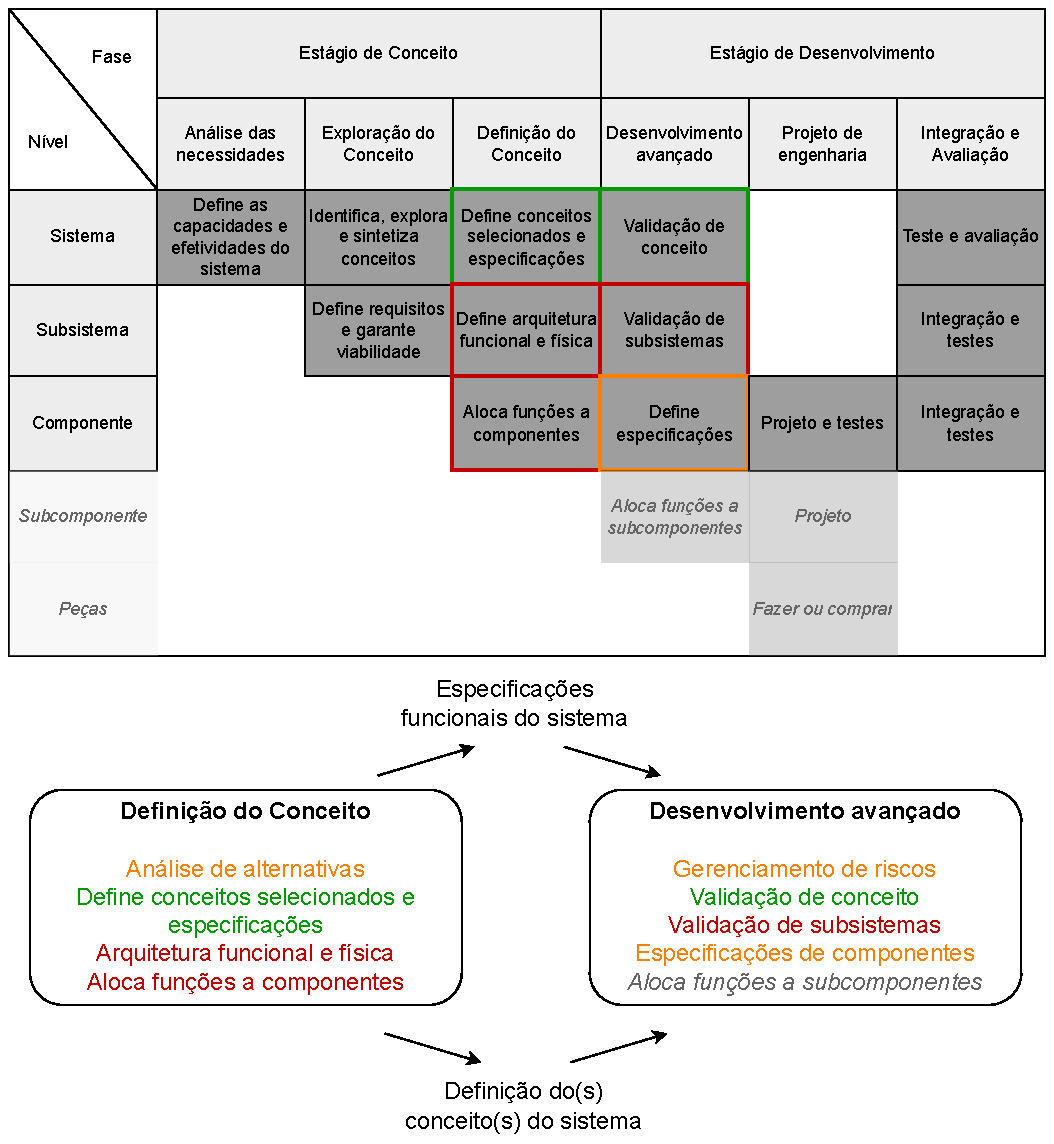
\includegraphics[width=0.8\textwidth]{./figuras/lifeCycleIssues.pdf}
		\caption{Destaque dos pontos falhos no ciclo de vida}
		\label{fig:metodologia:lifeCycleIssues}
	\end{figure}

	Em vermelho, temos as tarefas ou atividades que são completamente ignoradas nessas fases:
	\begin{itemize}
		\item Arquitetura física e funcional: Não é realizada a documentação da arquitetura do 
		sistema na fase de definição de conceito. Embora os desenvolvedores já possuam uma boa 
		noção de como seria o resultado final, a ausência desses artefatos impede a validação 
		dos subsistemas e a realização de um gerenciamento de riscos efetivo. Sem as arquiteturas 
		definidas, mesmo em alto nível, as outras partes interessadas não conseguem contribuir 
		adequadamente nas ponderações.
		\item Alocação de funções a componentes: Como não existe nenhuma das duas arquiteturas, 
		essa tarefa não é realizada. Essa tarefa seria justamente responsável por definir as 
		relações entre as arquiteturas, gerando assim uma forma de garantir a rastreabilidade do 
		sistema.
		\item Validação de subsistemas: Essa tarefa também não é realizada devido à falta da 
		documentação das arquiteturas do sistema. Essa deficiência constitui a raiz de algumas 
		falhas de entendimento dos requisitos, que acarretam a inclusão ou modificação de 
		funcionalidades no estágio de \textbf{Integração e avaliação}, afetando diretamente os 
		prazos estipulados.
	\end{itemize}

	Já em laranja, temos algumas atividades que são parcialmente realizadas no ciclo de vida atual:
	\begin{itemize}
		\item Análise de alternativas: Essa atividade é parcialmente realizada, pois acontece a discussão de alternativas com
		a área cliente durante a etapa de \textbf{Apresentação da linha do tempo}. Entretanto, não há a documentação das mesmas e, em alguns casos, uma melhor definição de conceito já descartaria opções
		inviáveis de serem implementadas.  
		\item Gerenciamento de riscos: Do ponto de vista gerencial ou estratégico, é realizado um gerenciamento de risco sucinto no que
		diz respeito aos prazos e marcos de entrega, novamente na etapa de \textbf{Apresentação da linha do tempo}. Por outro lado, na parte funcional e técnica, esse gerenciamento deixa a desejar. Como não
		há uma definição consistente e suficientemente detalhada, é incerto dizer quais são os possíveis pontos críticos ou que exigem maior atenção durante o desenvolvimento.
		Logo, não são planejadas ações para reduzir ou contornar os riscos envolvidos.
		\item Especificações de componentes: Essa tarefa está classificada como parcialmente realizada, pois era realizada simultaneamente com o desenvolvimento da solução na fase de \textbf{Projeto de Engenharia}.
		Semanalmente, as histórias de usuário eram detalhadas com as tarefas e especificações para serem realizadas na semana seguinte. Isso não permite uma validação prévia e, consequentemente, interfere também no gerenciamento de riscos.
		A realização dessa tarefa no momento correto interfere diretamente no bem-estar do projeto e da construção do sistema.
	\end{itemize}

	Por fim, em verde temos tarefas que são executadas de maneira satisfatória durante o ciclo de vida do sistema:
	\begin{itemize}
			\item Define conceitos selecionados e especificações: Ao observar a tabela de materialização do sistema, percebe-se que essa tarefa diz
			respeito ao primeiro nível, ou seja, são especificações e conceitos em nível de sistema, sem descer para níveis de maior detalhamento. Na
			etapa \textbf{Apresentação da linha do tempo} são apresentados possíveis cenários e alternativas criados anteriormente, como na etapa
			de \textbf{Estimativa de tarefas e esforço}, e é definido quais serão de fato considerados, bem como repassadas as suas especificações.
			\item Validação de conceito: Na mesma hierarquia, essa tarefa diz respeito à validação do conceito no nível de sistema, e isso 
			acontece também na etapa \textbf{Apresentação da linha do tempo}.
	\end{itemize}

	O fato de o sistema ser construído utilizando majoritariamente ferramentas de desenvolvimento \textit{low-code} faz com que exista um nível de abstração já intrínseco ao sistema.
	Dessa forma, durante as fases de \textbf{Desenvolvimento Avançado} e \textbf{Projeto de Engenharia}, não é necessário descer aos dois últimos níveis da hierarquia do sistema, ou seja,
	não são realizadas tarefas relacionadas aos subcomponentes ou às peças. Isso foi destacado na figura \ref{fig:metodologia:lifeCycleIssues}, com as duas últimas linhas da tabela esmaecidas
	e com a tarefa \textbf{Aloca funções a subcomponentes} em cinza na fase de \textbf{Desenvolvimento Avançado}.


	\section{Proposta de modificações}

	A partir do que foi apresentado nas seções anteriores, fica sugestivo que ações devem ser tomadas para que o ciclo de vida seja mais eficiente, focando nas fases de \textbf{Definição do Conceito} e
	\textbf{Desenvolvimento Avançado}.
	Na fase de definição de conceito faltam tarefas essenciais, que são dependências para a realização das tarefas da próxima fase. Elas são a criação das arquiteturas física e funcional, e a alocação de funções a componentes.
	
		
	\subsection{Arquitetura do Sistema}

	É necessário estipular um estilo de arquitetura com padrões que deverão ser seguidos e atualizados, de maneira que a equipe consiga 
	discutir o mesmo com as áreas clientes e entre sí, avaliando a qualidade estrutural e a escolha dos componentes do sistema. Tendo em vista que o tempo de vida do desenvolvimento
	do sistema é curto, padrões muito detalhados e que é necessário um grande esforço para criação não são interessantes para compor esse estilo de arquitetura.

	É proposto então a criação de dois artefatos de arquitetura, o primeiro seguindo um padrão que combina a arquitetura funcional com a lógica, baseado nas informações e requisitos obtidos
	para o sistema. Já o outro seguindo o padrão definido para a arquitetura física do sistema, de forma a documentar os componentes e subsistemas que serão responsáveis por cobrir as funcionalidades
	e lógicas definidas anteriormente.
	
	\subsubsection{Padrão para Arquitetura Funcional e Lógica}

	A documentação das arquiteturas funcionais e lógicas são importantes para a construção de uma boa arquitetura física e para a que a definição e validação de conceito seja assertiva. Como a 
	arquitetura funcional pode compor a arquitetura lógica, optou-se por unificar essas duas em únicos documentos, de maneira que seja otimizado o tempo empenhado para esse desenvolvimento.
	
	Esse padrão separa as funcionalidades em três grupos: Funcionalidades de Dados, Processos e Automações ou Documentos. Em cada grupo foram elencadas as funcionalidades básicas de um sistema genérico,
	representadas pelos retângulos preenchidos de azul. De cada uma dessas funcionalidades são derivados tópicos que elucidam o que deve ser documentado para expressar a lógica por trás
	da função de que derivam. As Figuras \ref{fig:metodologia:dataFunctionalities}, \ref{fig:metodologia:documetFunctionalities} e \ref{fig:metodologia:processFunctionalities} mostram esses grupos.

	\begin{figure}[!htb]
		\centering
		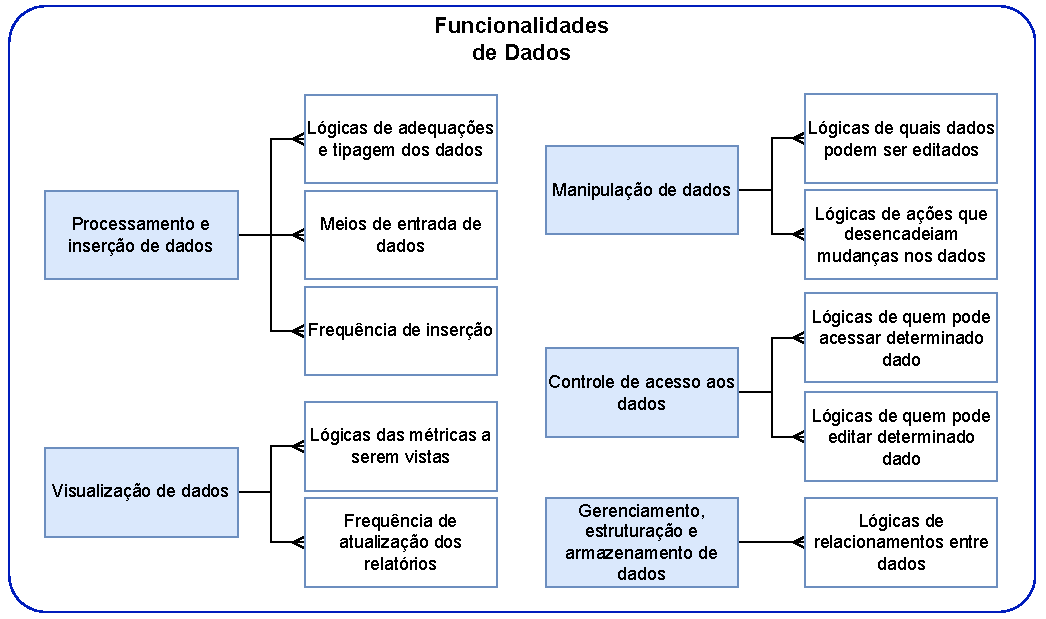
\includegraphics[width=1\textwidth]{./figuras/dataFunctionalities.pdf}
		\caption{Padrão de arquitetura funcional e lógica relacionadas aos dados.}
		\label{fig:metodologia:dataFunctionalities}
	\end{figure}

	\begin{figure}[!htb]
		\centering
		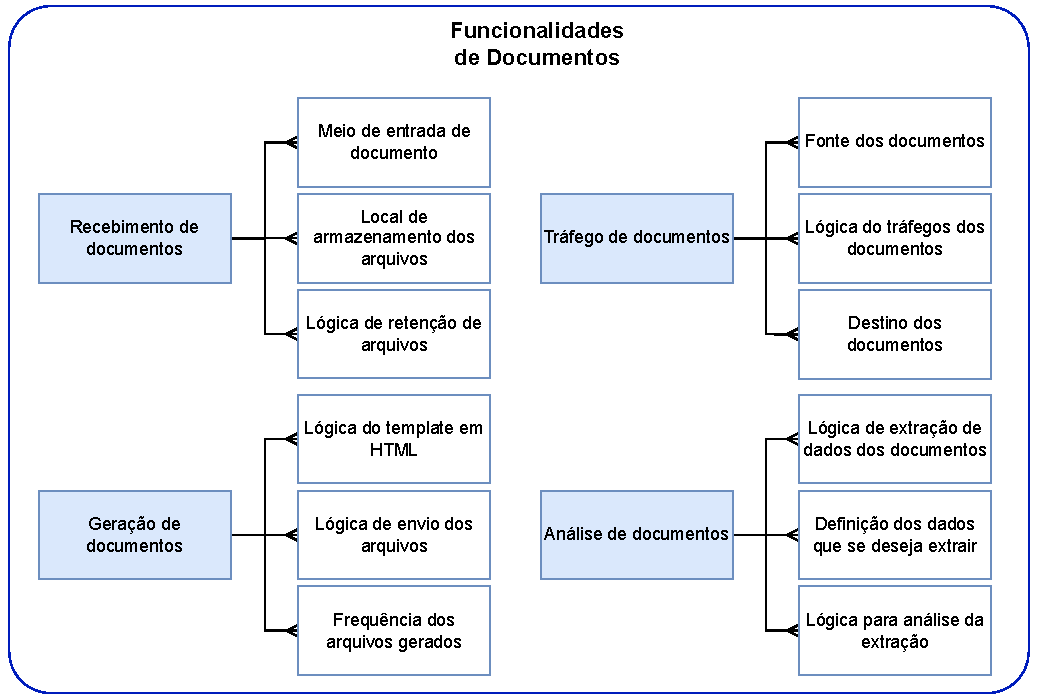
\includegraphics[width=1\textwidth]{./figuras/documetFunctionalities.pdf}
		\caption{Padrão de arquitetura funcional e lógica relacionadas a documentos.}
		\label{fig:metodologia:documetFunctionalities}
	\end{figure}

	\begin{figure}[!htb]
		\centering
		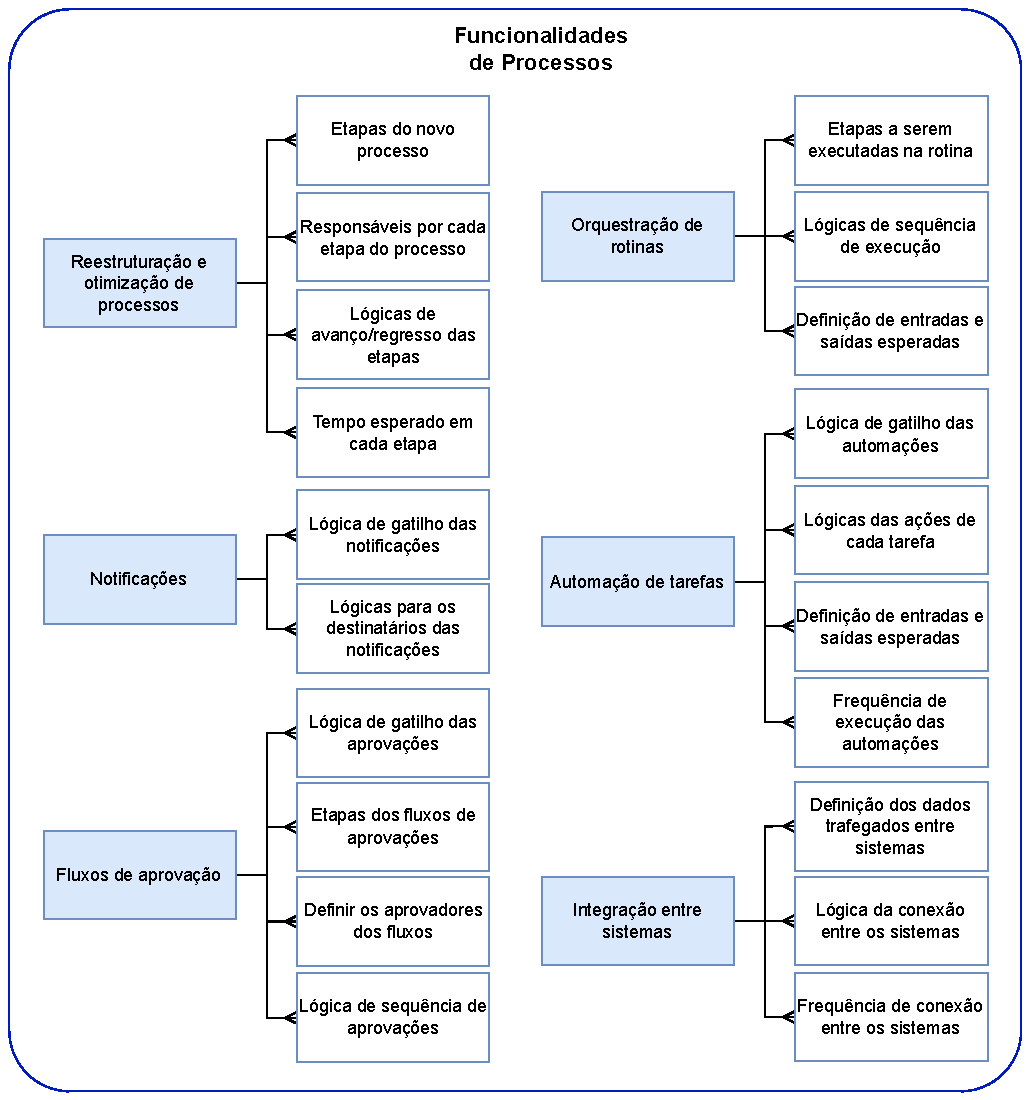
\includegraphics[width=1\textwidth]{./figuras/processFunctionalities.pdf}
		\caption{Padrão de arquitetura funcional e lógica relacionadas a processos e automações.}
		\label{fig:metodologia:processFunctionalities}
	\end{figure}

	Nesse padrão, não é definido com qual ferramenta ou tecnologia cada funcionalidade será implementada, pois isso será abordado posteriormente na arquitetura física. Cada sistema desenvolvido pode apresentar funcionalidades específicas não contempladas neste padrão devido às particularidades de cada projeto. Quando essas funcionalidades adicionais surgirem, elas devem ser incorporadas à documentação seguindo o mesmo padrão aqui estabelecido.

	\subsubsection{Padrão para Arquitetura Física}

	O padrão de arquitetura física proposto mantém um nível de detalhamento apropriado 
	para o contexto de desenvolvimento. A utilização de ferramentas \textit{low code} 
	permite essa simplificação sem comprometer a eficácia da documentação. Embora não 
	seja prática comum incluir modelos ou fornecedores específicos na documentação de 
	arquitetura física, o contexto já estabelecido da equipe de desenvolvimento 
	justifica a inclusão desses elementos nesta proposta.

	Os componentes do sistema são construídos utilizando majoritariamente as ferramentas disponíveis na \textit{Power Platform} sendo elas:

	\begin{itemize}
		\item \textit{Power Apps}: É uma ferramenta para o desenvolvimento ágil de aplicações personalizadas, utilizando pouco ou nenhum código. Ele permite que usuários construam interfaces gráficas
		interativas, conectadas a múltiplas fontes de dados, como o \textit{Dataverse}, SQL Server, Excel e SharePoint. Essa ferramenta é ideal para digitalizar processos manuais e implementar
		soluções específicas de negócios com rapidez e escalabilidade.

		\item \textit{Power Automate}: (anteriormente conhecido como Microsoft Flow) é uma ferramenta de automação de processos que permite criar fluxos de trabalho entre diferentes serviços e
		aplicações. É amplamente utilizado para automatizar tarefas rotineiras, como envio de notificações, aprovações de documentos, sincronização de dados entre sistemas e integração com APIs.

		\item \textit{Power BI}: É uma plataforma de \textit{Business Intelligence} que permite a criação de relatórios interativos e dashboards dinâmicos. Ele facilita a análise de dados provenientes
		de múltiplas fontes, promovendo a visualização e a tomada de decisões baseadas em evidências. Entre seus principais recursos estão: conexão com diferentes bancos de dados, uso de linguagem
		DAX para cálculos, compartilhamento de painéis e integração com outras ferramentas Microsoft.

		\item \textit{Copilot Studio}: Anteriormente conhecido como \textit{Power Virtual Agents}, é a ferramenta da Power Platform destinada à criação de assistentes virtuais e \textit{chatbots} com
		baixa ou nenhuma necessidade de codificação. Com sua nova abordagem centrada em IA generativa, permite desenvolver copilotos inteligentes capazes de interagir com usuários, acessar dados
		corporativos e executar ações automatizadas. É amplamente utilizado em cenários de atendimento ao cliente, suporte interno e automação de processos por meio de linguagem natural.

		\item \textit{Microsoft Dataverse}: Ou simplesmente \textit{Dataverse} é a plataforma de dados subjacente à Power Platform, projetada para armazenar, gerenciar e proteger dados empresariais estruturados. Ele fornece um modelo de
		dados comum, com suporte nativo a tipos de dados complexos, relacionamentos, regras de negócio, validações e integração com segurança do Microsoft Entra ID (antigo Azure AD). O Dataverse é
		fundamental para garantir consistência e integridade de dados em soluções desenvolvidas com o \textit{Power Apps}, \textit{Power Automate}, \textit{Power BI} e \textit{Copilot Studio}.
	\end{itemize}
	
	Na figura \ref{fig:metodologia:arquiteturaFisica} pode ser observado o padrão de arquitetura física sugerido para os sistemas desenvolvidos. Ela contém todos os possíveis
	elementos do sistema que podem ser utilizados para a arquitetura final de cada projeto executado bem como o agrupamento de subsistemas.
	\begin{figure}[h]
		\centering
		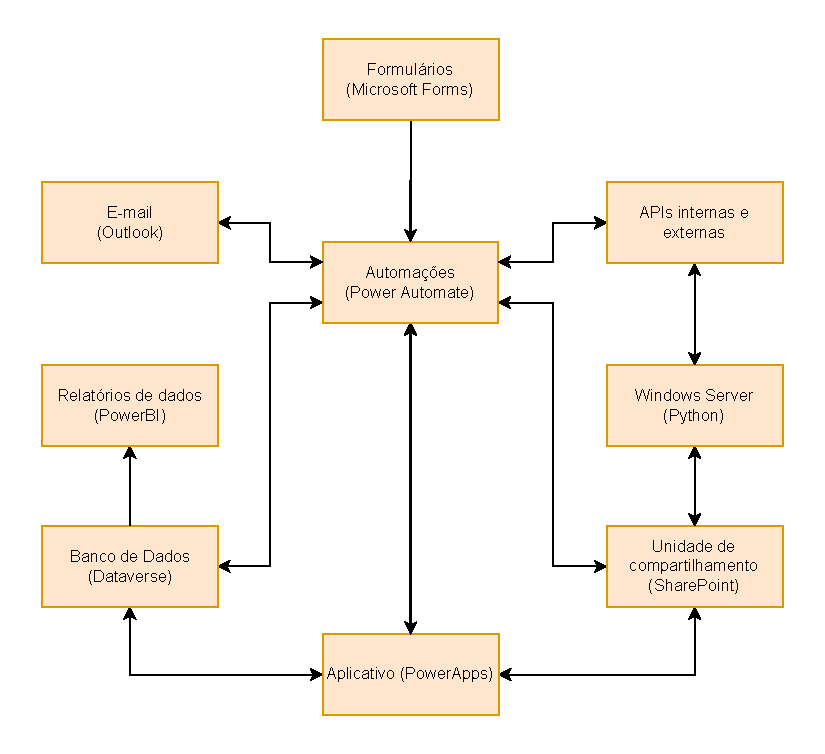
\includegraphics[width=1\textwidth]{./figuras/arquiteturaFisica.pdf}
		\caption{Padrão de arquitetura física dos sistemas desenvolvidos.}
		\label{fig:metodologia:arquiteturaFisica}
	\end{figure}
	
	Os Formulários são compomentes do sistema utilizados para coleta de dados e iniciar algum processo a partir de sua resposta. Sua utilização acontece principalmente quando existe
	o envolvimento de algum fornecedor ou cliente externo, pois são acessiveis sem necessidade de uma conta interna da empresa. Cada sistema ou subsistema pode utilizar um ou mais formulários.

	O E-mail ou mais especificamente uma caixa de e-mail compartilhada é um componente que pode ser utilizado tanto para comunicações e notificações do sistema quanto para recebimento de dados
	e arquivos por terceiros, visto que a possibilidade de anexo nos Fomulários são exclusivos quando o uso é estritamente interno. Normalmente cada sistema possui uma caixa compartilhada única
	para seus processos, mas há casos em que são necessária múltiplas caixas.

	Os Fluxos de Automação são o esqueleto da integração entre os subsistemas e sistemas externos. Cada Fluxo é um componente do sistema que realiza um conjunto de ações a partir de um gatilho.
	Esses fluxos são classificados em três tipos, e isso se dá pelo tipo de gatilho que os acionam.	Fluxos Agendados executam sua tarefas de maneira recorrente (a cada hora, diariamente,
	semanalmente, mensalmente ...) ou única a partir de uma data de início. Fluxos Instantâneos são acionados pela ação de um usuário em um aplicativo ou chat bot, ou são acionados por outros
	fluxos. Fluxos Automatizados utilizam conectores já disponíveis para serem acionados a partir de um evento em algum outro sistema, por exemplo, ser acionado quando um fomulário for respondido,
	quando um e-mail chegar na caixa de entrada, quando uma linha for criada em uma tabela no banco de dados, quando um arquivo for modificado, quando um acordo for assinado, etc. Exitem centenas
	de conectores disponíveis para diversos sistemas, aplicações e ferramentas.	Além disso, esses Fluxos de Automação são utilizados para consumir APIs que permitem métodos HTTP, criando assim 
	integrações com sistemas e ferramentas externas que não possuem conectores disponíveis mas que possuem API, bem como sistemas internos que foram criadas por outros times e que também tem
	uma API disponível que seja acessível pela internet.

	O Banco de Dados é um subsistema que armazena os dados do sistema, é relacional e necessita de uma modelagem e estruturação planejada, definindo os tipos dos dados de cada coluna nas tabelas,
	bem como os relacionamentos entre as tabelas criadas. Além disso, possui funcionalidades de gerenciamento de acesso aos dados.

	O Relatório de Dados apresentam gráficos, medidas e tendências, agrupados pelo nome de Visualizações, com o intuito de apresentar dados para decisões estratégicas de gestores. Os Relatórios
	são considerados subsistemas pois tanto	a manipulação dos dados quanto os cálculos para apresentar determinadas medidas podem levar a uma complexidade elevada. Este podem ser inseridos dentro
	de aplicativos e sites para uma facilidades de acesso aos usuários.

	As APIs Internas e Externas foram elencadas como componentes do sistema pois são essenciais para viabilizar o consumo e trafego de dados entre sistemas, atuando ainda como ponte entre sistemas
	locais e sistemas em nuvem.

	O Servidor é um subsistema que possui diversos Scripts que são executados localmente, principalmente códigos de RPA. O mesmo servidor suporta diversas áreas, onde as execuçòes são orquestradas
	para nao interferirem umas nas outras.

	A Unidade de Compartilhamento é um subsistema que é um serviço utilizado como um servidor de arquivos online. Possuem como componentes Bibliotecas de Documentos para armazenamento de arquivos relacionados
	a cada solução. Assim como no Banco de Dados, esse subsistema também possui funcionalidades de gerenciamento de acesso aos dados, no caso os documentos.

	O Aplicativo é um subsistema que abrange um diversa gama de funcionalidades e componentes. Entretanto, a quebra desses componentes ficou limitada apenas à documentação das telas do aplicativo,
	pois como já é utilizado uma ferramenta de \textit{low code} não traria muito valor descer ainda mais o nível de detalhamento. Para o Aplicativo também são definidos tipos de perfis de acesso
	aos dados, e também a determinadas telas ou funcionalidades.

	Os Agentes de IA são subsistemas que consultam Fontes de Dados como sites internos e externos, documentos e até Banco de Dados, e permitam que o usuário converse com um chat-bot do tipo RAG
	(Retrieval-Augmented Generation) que lhe responderá com base nas informações presentes nessas fontes selecionadas.

	\subsection{Rastreabilidade}

	Com as arquiteturas do sistema já definidas, cada elemento do sistema já possui suas funções e relacionamentos estabelecidos para acomodar as funcionalidades definidas para o sistema.
	Contudo, essa documentação pode não ser suficiente para definir de forma clara a interdependência dos elementos, visto que ela vai ser validada junto às áreas clientes e consequentemente tem um nível de detalhamento mais superficial.

	Assim, é proposto a criação de um aplicativo para registrar essa dependência entre componentes e trazer a rastreabilidade do sistema a um nível palpável para o time de desenvolvimento. Tendo como modelo o estilo e padrões de arquitetura sugeridos,
	nas Figuras \ref{fig:metodologia:appRastreabilidadeArqFunc} e \ref{fig:metodologia:appRastreabilidadeArqFis} vemos a proposta e conceito para esse aplicativo.

	\begin{figure}[!h]
		\centering
		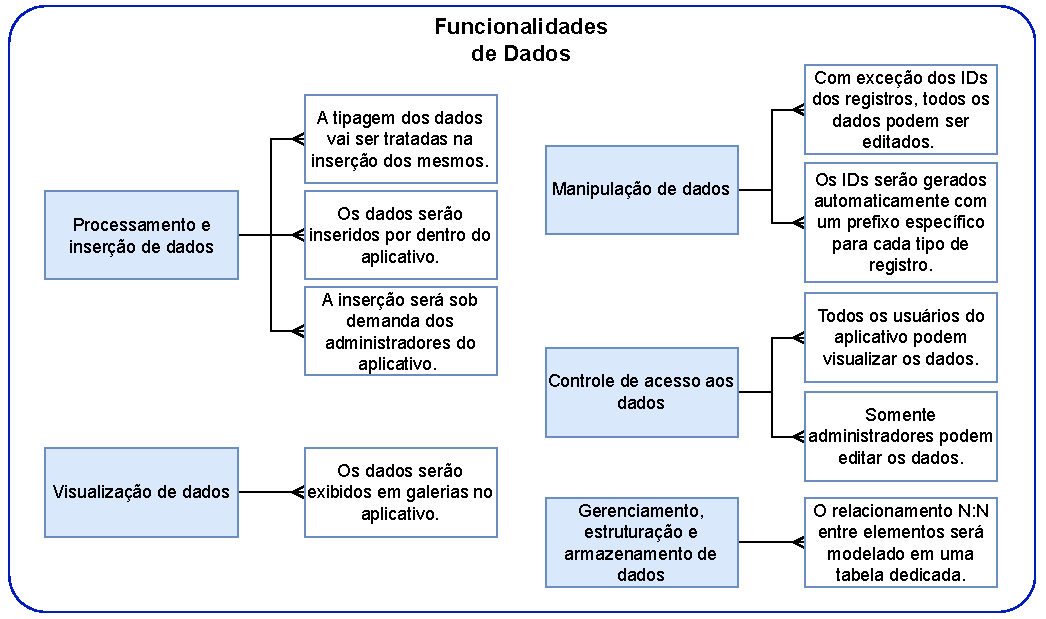
\includegraphics[width=1\textwidth]{./figuras/appRastreabilidadeArqFunc.pdf}
		\caption{Arquitetura funcional do aplicativo proposto}
		\label{fig:metodologia:appRastreabilidadeArqFunc}
	\end{figure}
	
	\begin{figure}[!h]
		\centering
		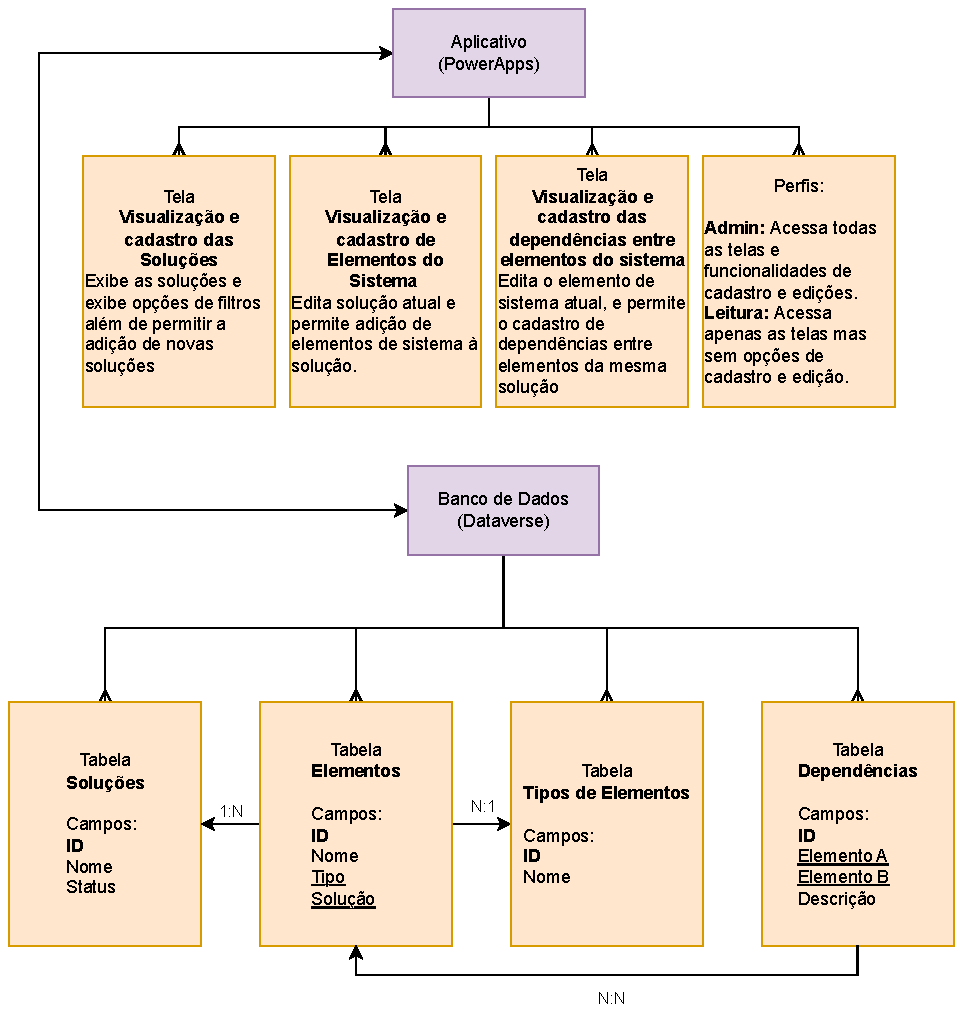
\includegraphics[width=0.85\textwidth]{./figuras/appRastreabilidadeArqFis.pdf}
		\caption{Arquitetura física do aplicativo proposto}
		\label{fig:metodologia:appRastreabilidadeArqFis}
	\end{figure}

	Nesse momento não há funcionalidades de Processos e Automações ou Documentos, o aplicativo é apenas uma forma de inserir e visualizar os dados de dependências entre os elementos.

	O aplicativo é simples e consiste em três telas onde são cadastradas e visualizadas as soluções desenvolvidas, os elementos de cada solução e a dependência entre os elementos de uma mesma solução.
	Os perfis separados são importantes para deixar a administração e cadastros de dependências com os desenvolvedores do time, mantendo no entanto a visibilidade para os gerentes de projeto e equipe.
	
	\section{Procedimentos para Coleta de Resultados}

	Com a intenção de trazer resultados quantitativos ao trabalho, são feitas comparações da percepção de esforço para a execução de tarefas em diferentes cenários e
	comparações com dados históricos de soluções desenvolvidas anteriormente pelo time. Além disso, uma avaliação do processo e dos ganhos nas relações com as áreas clientes, é realizada durante a rotina com as novas propostas sugeridas sendo aplicadas.

	\subsection{Comparação com Dados Históricos}

	Foi feito um levantamento das tarefas e esforços definidos anteriomente nas histórias de usuário para o desenvolvimentos dos elementos do sistema, separados em categorias,
	para as soluções já entregues e em produção, antes da aplicação das propostas apresentadas. Com isso, são definidas medidas estatísticas de Média de Pontos/Tarefas e Desvio Padrão de Pontos/Tarefas,
	onde cada tarefa recebeu pontos de esforço seguindo a sequência de Fibonacci.

	A relação das histórias de usuário, é composta pelo identificador na coluna ``ID'', seus dados de números de
	tarefas, os pontos de esforço totais extraídas da base histórica da equipe e foi adicionada ainda, na última coluna, a relação de ``(Pontos)/(Número de Tarefas)'' para ser
	utilizada nos cálculos das estatísticas a serem comparadas posteriormente com os novos dados a serem coletados.
	
	As estatísticas foram calculadas por categoria do tipo de desenvolvimento. Foi escolhida essa métrica de (Pontos)/(Número de Tarefas) para
	a análise, pois se trata de uma comparação que pode ser analisada mesmo entre categorias, e não é afetada pela complexidade do desenvolvimento, que seria o caso ao se analizar o número de tarefas ou
	o esforço total separadamente. Nesse caso é analisada a distribuição do esforço entre as tarefas, e como está esse comportamento em cada categoria.
	
	Após o desenvolvimento de novas soluções aplicando as propostas de arquitetura para a definição e validação de conceito, novos dados coletados vão compor os resultados a serem analisados e
	comparados com esse levantamento histórico.

	\subsection{Avaliação de cenários de manutenção}

	Com o intuito de avaliar o impacto da utilização do aplicativo proposto para garantir a rastreabilidade e mapear as dependências entre os elementos do sistema, três cenários de falha ou melhoria
	são analisados no que diz respeito ao esforço necessário para executá-lo.

	Para isso, soluções desenvolvidas no passado são cadastradas no aplicativo construído, bem como seus elementos e as dependências entre eles. E os outros desenvolvedores da equipe fazem essa estimativa
	duas vezes, a primeira apenas com a contextualização do cenário proposto e a outra com a utilização do aplicativo para consultar as dependências envolvidas em cada cenário.

	
	\section{Instrumentos e Materiais}

	A documentação do ciclo de vida atual do sistema, os fluxogramas e diagramas apresentados nesse trabalho, bem como os padrões de arquitetura propostos foram confeccionados
	na ferramenta online \textit{Draw.io}, 
	que além de gratuita para o desenho de diagramas de diferentes 
	tipos, não restringe o formato de salvamento do arquivo final, mantendo 
	assim a alta qualidade dos diagramas com imagens vetorizadas. 
	
	A aplicação será desenvolvida com as ferramentas e recursos disponíveis na \textit{Power Platform}. Para a interface de usuário será utilizado o \textit{Power Apps} e para a
	criação do banco de dados será utilizado o \textit{Dataverse}.

	Para a estimação de esforco das tarefas é utilizado uma extensão do aplicativo \textit{Azure DevOps} que habilita a funcionalidade de \textit{Planning Poker}, onde um desenvolvedor escolhe o esforço estimado
	sem ver a escolha dos outros, e depois todas as escolhas são reveladas simultaneamente, evitando assim a interferência na tomada de decisão alheia.
	